\documentclass[a4paper,11pt,oneside]{article}
%Dieses Dokument muss aufgrund der pst-circ-package mit XeLaTeX kompiliert werden

\usepackage[ngerman]{babel}	% Package für die einfache Darstellung von Umlauten
\usepackage{fancyvrb}
\fvset{fontsize=\normalsize}
\usepackage{cite}
\usepackage[obeyspaces]{url}
\usepackage[colorlinks=false,        % Links ohne Umrandungen in zu wählender Farbe
   linkcolor=black,   % Farbe interner Verweise
   filecolor=black,   % Farbe externer Verweise
   citecolor=black    % Farbe von Zitaten
]{hyperref}
\usepackage{algorithmic}
\usepackage{algorithm}
\usepackage{xcolor}
\usepackage{listings}
\usepackage{graphicx, epstopdf}
\usepackage{courier}
\usepackage{amsmath}
\usepackage{tabularx}
\usepackage{booktabs}
\usepackage{csquotes}
\usepackage{pst-circ}	% Package zum Zeichnen von Schaltplaenen (Achtung! Bei Nutzung mit Xelatex kompilieren)
\usepackage{float}
\usepackage{fancyhdr}
\usepackage{svg}		% Package zum Einbinden von svg-Dateien
%\usepackage{color}

\usepackage{upgreek}	% zusaetzliche griechische Zeichenbibliothek, Nutzung mit z.B. \uptau statt \tau
\usepackage[utf8]{inputenc}
\usepackage{trfsigns}	% Package zum Darstellen von Transformationszeichen

\usepackage[printonlyused]{acronym}		% Package für Abkürzungen

\fancyhf{}
\fancyhfoffset{0.5mm}
\fancyhead[L]{MTS}
\fancyhead[C]{Temperaturmessung mit PT100 und Thermoelement}
\fancyhead[R]{\thepage}

\fancyfoot[C]{Technische Hochschule L\"ubeck}


\setlength{\headheight}{15pt}

\usepackage{pdflscape}
\usepackage[onehalfspacing]{setspace}
\raggedbottom % Unterdr\"{u}ckt das Auseinanderziehen von Abs\"{a}tzen und setzt ein \clearpage stattdessen
\clubpenalty = 10000          
\widowpenalty = 10000
\displaywidowpenalty = 10000
\oddsidemargin = 0mm
\textwidth = 160mm
\topmargin = -5mm
\textheight = 225mm
\footskip = 60pt
\renewcommand{\footrulewidth}{.4pt}

\definecolor{mGreen}{rgb}{0,0.6,0}
\definecolor{mGray}{rgb}{0.5,0.5,0.5}
\definecolor{mPurple}{rgb}{0.58,0,0.82}
\definecolor{backgroundColour}{gray}{0.87}
\definecolor{CH1}{HTML}{e6e600}			% Vorgefertigte Farben fuer die Kanalfarben der Scopes
\definecolor{CH2}{HTML}{00e6e6}
\definecolor{CH3}{HTML}{e600e6}
\definecolor{CH4}{HTML}{00ed00}

\lstdefinestyle{CStyle}{						% Definition der Darstellung von C-Code
    backgroundcolor=\color{backgroundColour},   
    commentstyle=\color{mGreen},
    keywordstyle=\color{magenta},
    numberstyle=\tiny\color{mGray},
    stringstyle=\color{mPurple},
    basicstyle=\footnotesize\ttfamily,
    breakatwhitespace=false,         
    breaklines=true,                 
    captionpos=b,                    
    keepspaces=true,                 
    numbers=left,                    
    numbersep=5pt,                  
    showspaces=false,                
    showstringspaces=false,
    showtabs=false,                  
    tabsize=2,
    language=C
}

\usepackage[font=footnotesize,labelfont={color=cyan, bf}]{caption}

\usepackage{parskip}
\parskip 6pt plus 1pt minus 2pt % Zeilenabstand nach Absatz erh\"{o}hen
% \parindent 0pt                  % Einr\"{u}ckung auf "Standard" setzen

\usepackage{rotating}
\usepackage{enumitem}

\usepackage{rotating, graphicx}
\usepackage{caption}
%\usepackage{subcaption}
\usepackage{subfigure}

% \usepackage{hhline}
\usepackage{multirow}
\usepackage{dcolumn}
\newcolumntype{b}[1]{D{.}{\textbf{.}}{#1}}

\usepackage{tabularx}
\newcolumntype{L}[1]{>{\raggedright\arraybackslash}p{#1}} % linksb\"undig mit Breitenangabe
\newcolumntype{C}[1]{>{\centering\arraybackslash}p{#1}} % zentriert mit Breitenangabe
\newcolumntype{R}[1]{>{\raggedleft\arraybackslash}p{#1}} % rechtsb\"undig mit Breitenangabe

\usepackage[stable]{footmisc}

% Tikz Erweiterungen laden
\usepackage{pgf}
\usepackage{pgfplots}
\usepackage{tikz}

\pgfplotsset{compat=1.13}
\pgfdeclarelayer{background}
\pgfdeclarelayer{foreground}
\pgfsetlayers{background,main,foreground}

\tikzstyle{kasten} = [draw,outer sep=0,inner sep=5,minimum size=10]
\tikzstyle{kreis} = [circle,outer sep=0,inner sep=5,minimum size=10, draw=black]
\tikzstyle{punkt} = [circle, fill, draw=black, scale=0.4]
\tikzstyle{none}=[inner sep=3pt]
\usetikzlibrary{shapes,decorations.markings,arrows,positioning} 
\graphicspath{{pix/}} % Unterverzeichnisse
\fancypagestyle{Page_FH}{
  \fancyhf{}%
  \renewcommand{\headrule}{}%
  \fancyhfoffset{0.5mm}
  \setlength{\headheight}{110pt}
  \fancyhead[C]{%
    \begin{tikzpicture}%
      \begin{pgfonlayer}{foreground}%
        \node[] at (-1.45,0.2) {\begin{minipage}{0.7\textwidth}{Fachbereich Elektrotechnik und Informatik\\Bauelemente und Analoge Elektronik I}\end{minipage}};%
      \end{pgfonlayer}%
      \begin{pgfonlayer}{background}%
        \node[] at (0,0) {\includegraphics[width=0.98\textwidth]{pix/TH_Luebeck_Head.jpg}\hspace*{15pt}\color{white}.\hspace*{-16pt}};%
      \end{pgfonlayer}%
    \end{tikzpicture}}%
} 


\usepackage{makeidx}
\makeindex







%\documentclass[10pt,a4paper]{article}
%\usepackage[utf8]{inputenc}
%\usepackage[german]{babel}
%\usepackage[T1]{fontenc}
%\usepackage{amsmath}
%\usepackage{amsfonts}
%\usepackage{amssymb}
%\usepackage[left=3cm,right=3cm,top=3cm,bottom=2cm]{geometry}
\author{von Roman Weber, Chris Klobke\\Betreuer: Prof. Dr.-Ing. Jochen Abke, Joachim Kaczmareck}
\title{Messtechnik und Sensorik\\Temperaturmessung mit PT100 und Thermoelement}
\date{14. November 2019}

%\usepackage{graphicx}

%\usepackage{fancyhdr}
%\pagestyle{fancy}
%\fancyhead{}
%\fancyfoot{}
%\fancyhead[L]{MTS}
%\fancyhead[C]{Versuch 2}
%\fancyhead[R]{\thepage}
%\fancyfoot[C]{Technische Hochschule Lübeck}
%\renewcommand\headrulewidth{0.5pt} 			 
%\renewcommand\footrulewidth{0.5pt}  	

		
\begin{document}
\pagestyle{empty}

Fachbereich Elektrotechnik und Informatik \\
Messtechnik und Sensorik
%%\\


\begin{center}

\LARGE\textbf{Temperaturmessung mit PT100 und Thermoelement} \\
\LARGE\textbf{Praktikumsversuch 1} \\
\LARGE\textbf{WiSe 19/20} \\

\vspace{2.0cm}

\end{center}

\vspace{5.0cm}

\begin{tabular}{lll}
  Autor(en): & Chris Klobke & (chris.klobke@stud.th-luebeck.de) \\
  			 & Roman Weber & (roman.weber@stud.th-luebeck.de) \\
  Betreuer: & Prof. Dr.-Ing. Jochen Abke & (jochen.abke@th-luebeck.de) \\
  			& Joachim Kaczmareck & (joachim.kaczmareck@th-luebeck.de) \\
  Version: & 1.0 & \\
  Versuchstermin: & 14. November 2019 & \\
\end{tabular}

\vspace{1.0cm}


\vspace{2.0cm}
\begin{table}[h]
\centering
%\resizebox{\textwidth}{!}{%
\begin{tabular}{|c|c|c|}
\hline
\textbf{Bericht abgegeben am:} & \textbf{zu korrigieren bis:} & \textbf{testiert am:} \\ \hline
\rule{0pt}{1.0cm}  &  & \multirow{2}{*}{} \\ \cline{1-2}
\rule{0pt}{1.0cm}  &  & \rule{4cm}{0cm} \\ \hline
\end{tabular}%
%}
\end{table}
\newpage
\tableofcontents
\pagestyle{fancy}
\newpage
\section{Vorbereitung}
\subsection{Aufgabenstellung}
Zur Vorbereitung liegt die Aufgabe erstens darin, den Widerstand des Pt100 bei einer angenommenen Raumtemperatur von $25^ \circ C$ und zweitens die Spannung des Thermoelements bei selbiger Temperatur zu ermitteln.
\subsection{Durchführung und Messergebnisse}
a)\\
Mithilfe der Taylorreihe und den Temperaturkoeffizienten des Pt100, $\alpha = 3,90802   \cdot 10^{-3} {}^\circ C^{-1}$ und $\beta = -5,80195 \cdot 10^{-7} {}^\circ C^{-2}$, lässt sich der Widerstandswert des Pt100 bei einer Temperatur von $T = 25^\circ C$ bestimmen.

\begin{center}
$R_t = R_0 \cdot (1 + \alpha \cdot T + \beta \cdot T^2)$ \\
$R_t = 100 \Omega \cdot (1 + 3,90802 \cdot 10^{-3} {}^\circ C^{-1} - 5,80195 \cdot 10^{-7}{}^\circ C ^{-2} \cdot 25 ^\circ C ^2)$ \\
$R_t = 109,734 \Omega$
\end{center}
b)\\
Da die Kirchhoffsche Maschenregel besagt, dass die Summe aller Teilspannungen null ergibt, lässt sich für die Masche eines Thermoelements folgende Gleichung aufstellen: 
\begin{center}
$U_{A,B} + k_{B,A} \cdot T_M = 0$
\end{center}
$k_{A,B} \cdot T_M$ ergibt hierbei das Spannungspotential zwischen den beiden Metallen des Thermoelements.\\
Nach Umstellen lässt sich die Spannung $U_{A,B}$ bestimmen.
\begin{center}
$U_{A,B} = k_{A,B} \cdot T_M = \frac{4,095mV}{100K} \cdot 25^\circ C = 1,024mV$
\end{center}

\newpage

\section{Widerstandsthermometer}
\subsection{Aufgabenstellung}
Beim ersten Versuch besteht die Aufgabe daraus, die Widerstandswerte der vorhandenen zwei Pt100-Widerstandsthermometer bei gegebenen Umgebungstemperaturen zu messen. Zur Temperatur-Regulation steht ein Kalibrierofen zur Verfügung. \\
\subsection{Versuchsaufbau}
Die beiden Widerstandsthermometer (Pt 100 Ref und Pt 100) werden im Ofen platziert. Der kalibrierte Referenz-Pt100 wird mit einer Vierleitertechnik am Multimeter angeschlossen, der unkalibrierte Pt100 mit einer Zweileitertechnik. \\ 
Der Referenz-Pt100 dient hierbei zur exakten Bestimmung der Temperatur innerhalb des Ofens.

\begin{figure}[h]
\centering
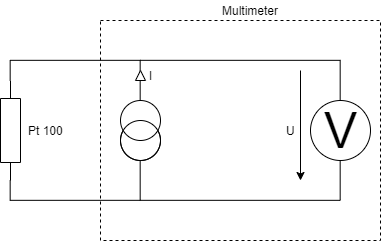
\includegraphics[scale=0.5]{Bilder/Aufg1Schaltbild1.png}
\caption{Zweileitertechnik}
\end{figure}

\begin{figure}[h]
\centering
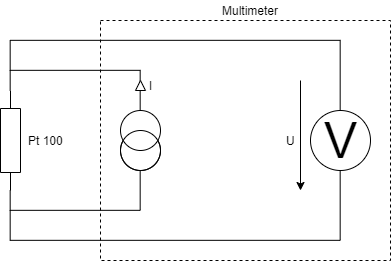
\includegraphics[scale=0.5]{Bilder/Aufg1Schaltbild2.png}
\caption{Vierleitertechnik}
\end{figure}



\newpage
\subsection{Durchführung}
Als erstes werden die Widerstandswerte der beiden Widerstandsthermometer bei Raumtemperatur aufgenommen. Anschließend wird die Temperatur innerhalb des Ofens so eingestellt, dass neben des Widerstandswertes bei Raumtemperatur, Werte zwischen $60^\circ C$ und  $300^\circ C$ in Schritten von $\Delta T = 60K$ aufgenommen werden können. 
\subsection{Messergebnisse}
Die Messwerte sind folgendem Diagramm und der Tabelle zu entnehmen. \\
\begin{center}
\begin{tabular}{|c|r|r|r|}
\hline 
T Ist/$^\circ C$ & Pt 100 Ref/$\Omega$ & Pt 100/$\Omega$ & Regression/$\Omega$ \\ 
\hline 
21,119 & 108,244 & 109,133 & 110,770 \\ 
\hline 
61,556 & 123,843 & 124,865 & 125,744 \\ 
\hline 
120,833 & 146,397 & 147,493 & 143,991 \\ 
\hline 
180,624 & 168,735 & 170,016 & 169,835 \\ 
\hline 
241,030 & 190,883 & 191,949 & 192,203 \\ 
\hline 
301,233 & 212,537 & 213,621 & 214,497 \\ 
\hline 
\end{tabular} 
\end{center}
\begin{figure}[h]
\centering
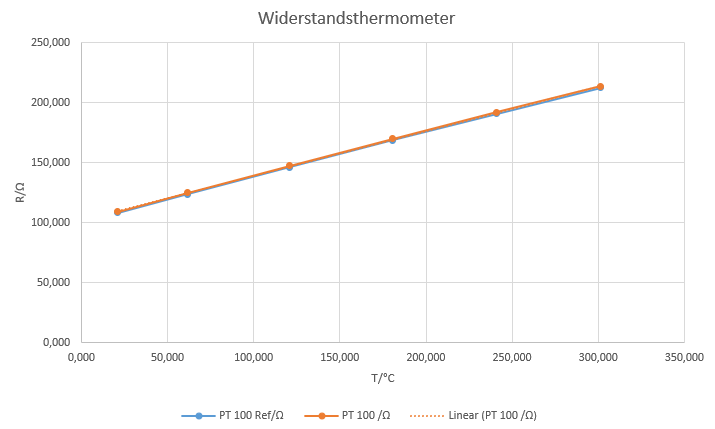
\includegraphics[scale=0.8]{Bilder/Aufg1Diagramm.png}
\caption{Pt 100 Messwerte}
\end{figure}
\newpage

Regressionsgerade:
\begin{center}
$R(T) = a + bT = 101,91 + 0,3731 \frac{\Omega}{{}^\circ C} \cdot T$
\end{center}
Der Parameter a steht hierbei für den Widerstandswert der Regression bei $T = 0^\circ C$. \\
m ist bei linearem Verlauf die Empfindlichkeit. Somit steigt die Regression des Widerstands des Pt100 um $\frac{0,3731 \Omega}{1 ^\circ C}$. 
\\\\
Mithilfe der Regressionsgeraden lässt sich ein Bestimmtheitsmaß $R^2$ ermitteln. 
\begin{center}
$R^2 = 0,9998$
\end{center}
Linearitätsfehler:
\begin{center}
$F_{Lin} = \frac{R_{Messung}(T) - R_{Regression}(T)}{R_{Messung}(T_{max}) - R_{Messung}(T_{min})}\cdot 100\%$\\
\vspace{0.5cm}
$F_{Lin} = \frac{170,016\Omega - 169,301 \Omega}{213,621\Omega - 109,133\Omega}\cdot 100\%$\\
\vspace{0.5cm}
$F_{Lin} = 0,684 \%$
\end{center}

Folgend ist der Linearitätsfehler in Abhängigkeit der Temperatur als geglättete Funktion zu erkennen.
\begin{figure}[h]
\centering
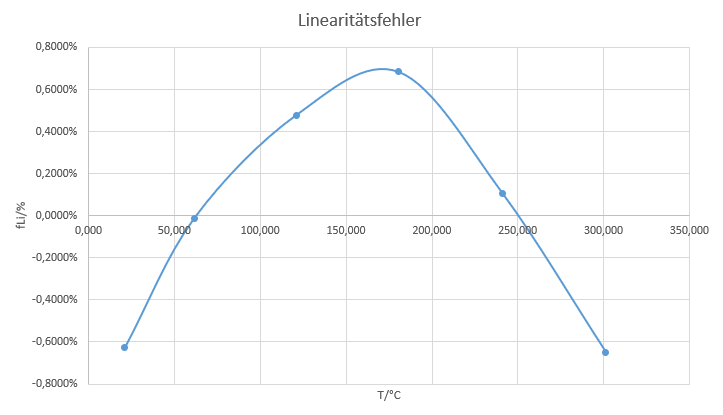
\includegraphics[scale=0.8]{Bilder/Aufg1Diagramm2Gegl.png}
\caption{Fehlerkennlinie}
\end{figure}

\newpage

Berechnung der Konstanten:\\
Zur Bestimmung der Konstanten der Widerstandsthermometer wird folgendes Polynom betrachtet:

\begin{center}
$R_t = R_0 \cdot (1 + \alpha \cdot T + \beta \cdot T^2)$
\end{center}

Da bei niedrigen Temperaturen der quadratische Term zu vernachlässigen ist, erschließt sich daraus folgende Gleichung:

\begin{center}
$R_t = R_0 \cdot (1 + \alpha \cdot T)$
\end{center}
 
Mit den zwei niedrigsten Temperaturen der gemessenen Werte können zwei Gleichungen erstellt und somit das $\alpha$ errechnet werden. 

\begin{center}
$\alpha = 3,855 \cdot 10^{-3}$
\end{center}

Anhand dieses Alphas lässt sich anschließend $R_0$ bestimmen.

\begin{center}
$R_0 = \frac{R}{1 + \alpha T} = \frac{124,865\Omega}{1 + 3,855 \cdot 10^{-3} \cdot 61,5564^\circ C}$\\
\vspace{0.5cm}
$R_0 = 100,917^\circ C$
\end{center}

Mithilfe von $R_0$ und $\alpha$ lässt sich $\beta$ bestimmen. Bei der folgenden Gleichung entspricht $T_{300} = 301,233^\circ C$.
\begin{center}
$\beta = \frac{R_{300} - R_0(1+\alpha \cdot T_{300})}{R_0 \cdot T_{300}^2}$\\
\vspace{0.5cm}
$\beta = \frac{213,621 \Omega - 100\Omega (1+ 3,855\cdot 10^{-3} \cdot 301,233)}{213,621 \cdot 301,233^2}$\\
\vspace{0.5cm}
$\beta = -1,2919 \cdot 10^{-7}$
\end{center}

Mit dem selbigen Verfahren lassen sich diese Konstanten ebenfalls für den Pt100-Ref bestimmen. Die Konstanten für beide Widerstandsthermometer werden in der folgenden Tabelle dargestellt.\\
\begin{center}
\begin{tabular}{|c|r|r|r|}
\hline 
 & $R_0 / \Omega$ & $\alpha/^\circ C^{-1}$ & $\beta / ^\circ C ^{-2}$ \\ 
\hline 
Datenblatt & 100 & $3,9080 \cdot 10 ^{-3}$ & $-5,80195 \cdot 10^{-7}$ \\ 
\hline 
PT100 & $100,917$ & $3,855 \cdot 10^{-3}$ & $-1,2319 \cdot 10^{-7}$ \\ 
\hline 
PT100 Ref & $100,066$ & $3,86 \cdot 10^{-3}$ & $-1,9390 \cdot 10^{-7}$ \\ 
\hline 
\end{tabular} 
\end{center}
\newpage

\subsection{Fazit}
Wie zu erwarten, ist das kalibrierte Referenz-Widerstandsthermometer Pt100-Ref genauer als der nicht kalibrierte Pt100. Grund hierfür ist unter anderem, der Einsatz der Zweileitertechnik beim nicht kalibrierten Pt100, während beim Pt100-Ref die Vierleitertechnik zum Einsatz kommt. \\
Zu erkennen ist dies vor allem an den konstanten Temperaturkoeffizienten, da sowohl $R_0$, als auch $\alpha$ des kalibrierten Widerstandsthermometer nur gering von den aus dem Datenblatt angegebenen Konstanten abweicht. Auch die Werte des nicht kalibrierten Pt100 weichen nur leicht von den idealen Werten ab. Ein Unterschied zum kalibrierten ist jedoch gerade bei den dargestellten Messwerten zu erkennen. Die Zweileitertechnik weist dort eine leicht positive Differenz zu jedem Idealwert auf. Grund dafür ist der in der Zweileitertechnik relevante Leitungswiderstand.\\\\
Außerdem zu erkennen ist, dass die Konstante $\beta$ bei beiden Widerstandsthermometern stark vom Idealwert abweicht. Das liegt daran, dass der quadratische Koeffizient bei, in diesem Versuch vorkommenden Maximaltemperaturen, kaum eine Rolle spielt. Dieser ist jedoch vor allem bei höheren Temperaturen bis zu $850^\circ C$ relevant. 

\section{Thermoelement}
\subsection{Aufgabenstellung}
Bei diesem Versuch sollen die Spannungen des Thermoelements bei gegebenen Temperaturen aufgenommen werden. Zur Temperatur-Regulation steht auch hier ein Kalibrierofen zur Verfügung. 
\subsection{Versuchsaufbau}
Das Thermoelement befindet sich auch hier zu Beginn des Versuchs im Kalibrierofen. Dieses Thermoelement ist über zwei Leiterkabel direkt an das Digitalmultimeter angeschlossen. \\
\begin{figure}[h]
\centering
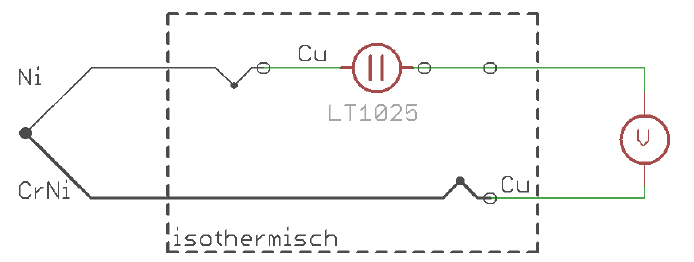
\includegraphics[scale=0.7]{Bilder/Aufg2Schaltbild1.png}
\caption{Thermoelement Schaltbild}
\end{figure}

\newpage

\subsection{Durchführung}
Zu Beginn des Versuchs wird die Spannung am Thermoelement bei Raumtemperatur aufgenommen. Die Temperatur im Ofen wird mit $\Delta T = 60K$ erhöht und die Thermospannungen aufgenommen. 
\subsection{Messergebnisse}
Die aufgenommenen Messwerte sind dem folgenden Diagramm und der Tabelle zu entnehmen.

\begin{center}
\begin{tabular}{|c|r|r|}
\hline 
T Ist/$^\circ C$ & Thermo/mV & Regression/mV \\ 
\hline 
21,119 & 0,842 & 0,890 \\ 
\hline 
61,556 & 2,520 & 2,527\\ 
\hline 
120,833 & 4,986 & 4,928\\ 
\hline 
180,624 & 7,378 & 7,350\\ 
\hline 
241,030 & 9,756 & 9,796\\ 
\hline 
301,233 & 12,200 & 12,234\\ 
\hline 
\end{tabular} 
\end{center}

\begin{figure}[h]
\centering
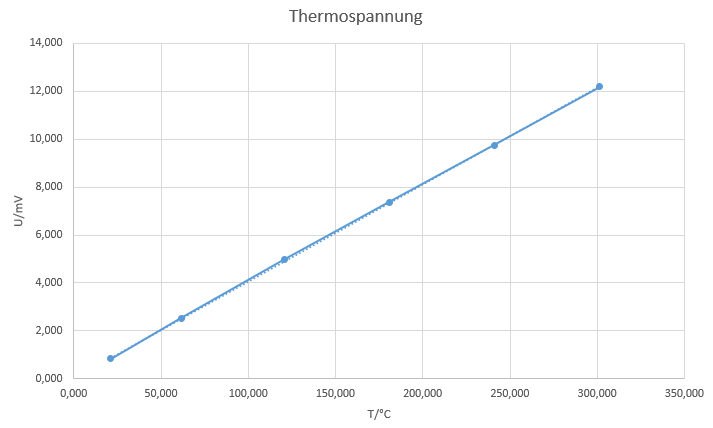
\includegraphics[scale=0.8]{Bilder/Aufg2Diagramm.png}
\caption{Thermoelement Spannungskennlinie}
\end{figure}

Regressionsgerade:
\begin{center}
$U_{th}(T) = U_{th}(T=0^\circ C) + a \cdot T$
$U_{th}(T) = 0,0344 + 0,0405 \cdot T$
\end{center}

Der Parameter $U_{th}$ steht hierbei für die Thermospannung bei einer Temperatur von $T = 0^\circ C$, während a die Empfindlichkeit der Regressionsgeraden angibt. Die Empfindlichkeit der Thermoelement-Regressionsgeraden beträgt $\frac{0,0405 mV}{1 ^\circ C}$.

\newpage

Linearitätsfehler:

\begin{center}
$F_{Lin} = \frac{U_{Messung}(T) - U_{Gerade}(T)}{U_{Messung}(T_{max}) - U_{Messung}(T_{min})}\cdot 100\%$\\
\vspace{0.5cm}
$F_{Lin} = \frac{4,986mV - 4,928mV}{12,200mV-0,842mV}\cdot 100\%$\\
\vspace{0.5cm}
$F_{Lin} = 0,511\%$
\end{center}

\subsection{Fazit}
Zu erkennen ist, dass sowohl der Pt100 als auch das Thermoelement ihre größten Abweichungen zur Regression im mittleren Temperaturbereich besitzen ($120^\circ C - 140^\circ C$). Bei einer Temperatur von $120^\circ C$ ist die Abweichung des Thermoelements mit 0,511\% sogar großer als die des Pt 100 (0,479\%). Ansonsten ist das Thermoelement jedoch, vor allem im höheren Temperaturbereich, deutlich genauer.
\newpage

\section{Einfluss des Leitungswiderstandes}
\subsection{Aufgabenstellung}
In diesem Versuch wird untersucht wie sich der Leitungswiderstand auf die Zweileiter- bzw. Vierleitertechnik und die Direktmessung auswirkt.
\subsection{Versuchsaufbau}
Im ersten Teil der Aufgabe wird eine Wheatstonsche Brücke mit Zweileitertechnik und dem Pt100-Simulator anstatt eines Pt100 aufgebaut.
\begin{center}
\begin{figure}[h]
\centering
\includegraphics[scale=0.4]{Bilder/WheatstonscheBrücke.png}
\caption{Wheatstonsche  Brücke mit Zweileitertechnik}
\end{figure}
\end{center}

\newpage

Um herauszufinden welchen Einfluss die Leitungswiderstände $R_L$ auf die Messung haben, werden diese durch stufenweise einstellbare Widerstände simuliert. \\\\
\vspace{1cm}
\begin{figure}[h]
\centering
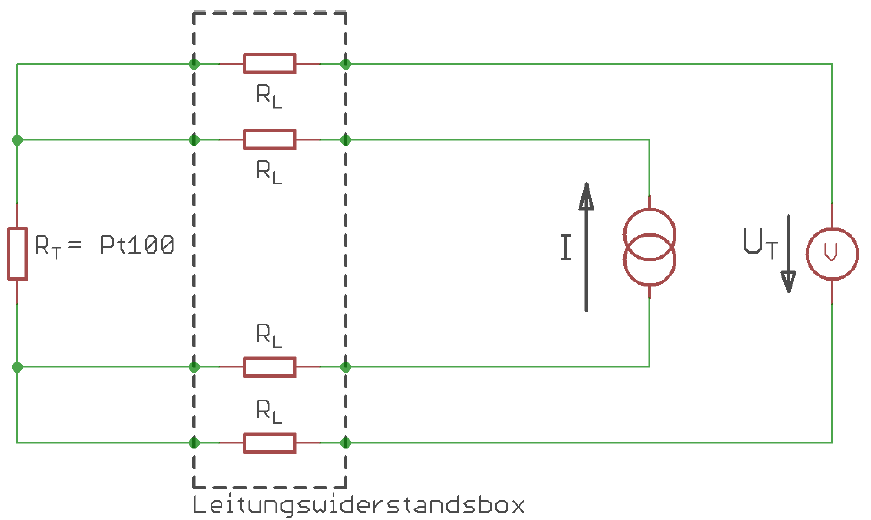
\includegraphics[scale=0.5]{Bilder/4Leitertechnik.png}
\caption{Vierleitertechnik}
\end{figure}

\begin{figure}[h]
Im letzten Teil der Aufgabe wird dann der Pt100-Simulator mit der Vierleitertechnik direkt an das digitale Multimeter angeschlossen.\\
\end{figure}

\begin{figure}[h]
\centering
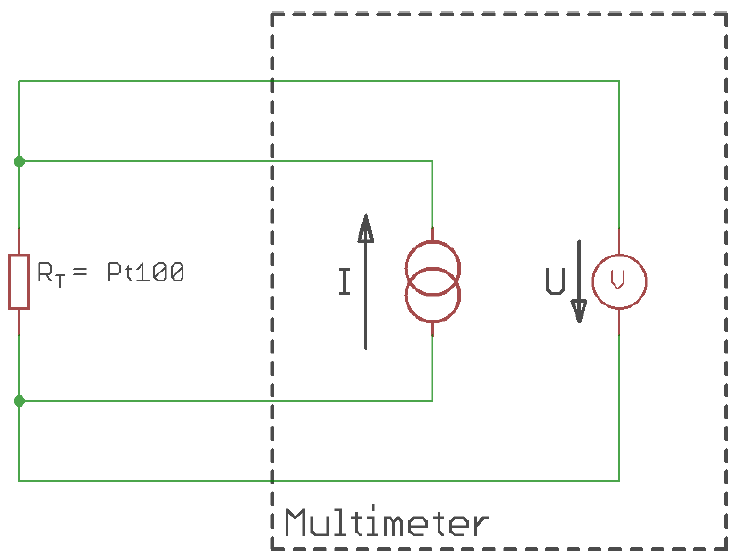
\includegraphics[scale=0.4]{Bilder/4LTDIMM.png}
\caption{Widerstandsmessung mit dem Multimeter}
\end{figure}

\newpage

\subsection{Durchführung}
Nach korrektem Aufbau der Wheatstonschen Messbrücke wird die Spannungsspeisung $U_0$ auf 0V und der PT100-Simmulator auf $100^\circ C$ eingestellt. Als nächstes werden die Potentiometer, die die Leitungswiderstände simulieren, auf $0\Omega$ eingestellt. Zu dem Zeitpunkt wird die Brückenspannung notiert. Die Potentiometer werden daraufhin auf $ 1\Omega; 5,1\Omega; 10\Omega $ und $ 22,1\Omega$ eingestellt.\\
Nach erfolgreicher Messung wird anschließend die Vierleitertechnik  aufgebaut und die Stromspeisung auf $I_0=10mA$ eingestellt. Daraufhin werden dann die Potenziometer wie beim Aufgabenteil zuvor erhöht und die Messwerte aufgenommen.\\
Die Messung mit dem Pt100-Simulator direkt am Multimeter wird auf die selbe Art und Weise durchgeführt. 
\subsection{Messergebnisse}
Die aufgenommenen Messwerte werden in der folgenden Tabelle Dargestellt.\\
\begin{center}
\begin{tabular}{|c|r|r|r|}
\hline 
$R_L/\Omega $ & $U_{B}$/mV & $U_{T}$/V & DMM/$\Omega$ \\ 
\hline 
0 & 167,203 & 1,385 & 138,412 \\ 
\hline 
1 & 170,564 & 1,385 & 138,412 \\ 
\hline 
5,1 & 198,582 & 1,385 & 138,412 \\ 
\hline 
10 & 228,791 & 1,385 & 138,413 \\ 
\hline 
22,1 & 293,792 & 1,385 & 138,421 \\ 
\hline 
\end{tabular} 
\end{center}
\vspace{1cm}
Um nun aus den gemessenen Spannungen die Widerstandswerte zu berechnen werden volgende Formeln benötigt:\\\\
Wheatstonschen Brücke:\\
\begin{center}
$R(PT100)= \frac{U_0+2U_B}{U_0-2U_B}\cdot 100\Omega$

\end{center}
4-Leitertechnik:\\
mit $R=100\Omega$\\
\begin{center}
$R=\frac{U_T}{I}$
\end{center}
Die Ergebnisse dieser Rechnungen sind in der folgenden Tabelle dargestellt.\\
$R_B$ entspricht dem Wert der Wheatstonschen Brück und $R_T$ entspricht dem Wert der Vierleitertechnik.
\begin{center}
\begin{tabular}{|c|r|r|}
\hline 
$R_L/\Omega$ & $R_B/\Omega$ & $R_T/\Omega$ \\ 
\hline 
0 & 140,155 & 135,5 \\ 
\hline 
1 & 141,128 & 135,5 \\ 
\hline 
5,1 & 149,558 & 135,5 \\ 
\hline 
10 & 159,333 & 135,5 \\ 
\hline 
22,1 & 183,203 & 135,5 \\ 
\hline 
\end{tabular} 
\end{center}
Um nun die entsprechenden Temperaturen der Widerstandswerte zu errechnen muss die folgende quadratische Gleichung nach T umgestellt werden.\\
\begin{center}
$R_T=R_0(1+\alpha \cdot T+\beta \cdot T^2)$\\


\end{center}
Die errechneten Temperaturwerte werden in folgender Tabelle dargestellt.
\begin{center}
\begin{tabular}{|c|r|r|r|}
\hline 
$R_L/\Omega$ & $T_B/^\circ C$ & $T_T/^\circ C$ & $T_{DMM}/^\circ C$ \\ 
\hline 
0 & 104,367& 92,098 & 99,768 \\ 
\hline 
1 & 106,938 & 92,098 & 99,768 \\ 
\hline 
5,1 & 129,293 & 92,098 & 99,768 \\ 
\hline 
10 & 155,409 & 92,098 & 99,771 \\ 
\hline 
22,1 & 220,095 & 92,098 & 99,792 \\ 
\hline 
\end{tabular} 
\end{center}
\vspace{1cm}
Anhand dieser Temperaturwerte und der folgenden Formel lassen sich die jeweiligen Messfehler errechnen.\\
Diese sind in der nachstehenden Tabelle zu entnehmen.
\begin{center}
$F(R_L)=\frac{T'(RL)-100^\circ C}{100^\circ C}\cdot 100\%$
\end{center}
\vspace{1cm}
\begin{center}
\begin{tabular}{|c|r|r|r|}
\hline 
$R_L$ & $F_B/\%$ & $F_T/\%$ & $F_{DDM}/\%$ \\ 
\hline 
0 & 4,367 & -7,902 & -0,232 \\ 
\hline 
1 & 6,938 & -7,902 & -0,232 \\ 
\hline 
5,1 & 29,293 & -7,902 & -0,232 \\ 
\hline 
10 & 55,409 & -7,902 & -0,229 \\ 
\hline 
22,1 & 120,095 & -7,902 & -0,208 \\ 
\hline 
\end{tabular} 
\end{center}
\newpage
Die Messabweichungen sind außerdem im folgenden Diagramm grafisch dargestellt.
\begin{figure}[hbtp]
\centering
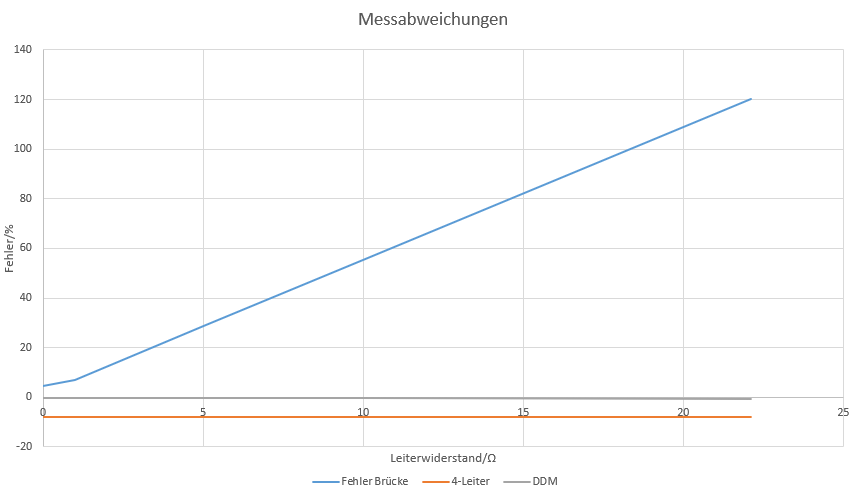
\includegraphics[scale=0.7]{Bilder/Diagramm_Messabweichungen.png}
\caption{Messabweichungen}
\end{figure}



\subsection{Fazit}
An diesem Versuch ist sehr gut zu erkennen, dass die Messabweichungen bei der Zweileitertechnik im Gegensatz zur Vierleitertechnik bei steigendem Leitungswiederstand stark steigen. Die Messwerte bei der Vierleitertechnik hingegen bleiben bis auf die dritte Nachkommastelle gleich. Wenn der Messwiederstand jedoch direkt an das Multimeter angeschlossen wird, ist eine minimale Änderung des Messfehlers zu bemerken. Dies ist dadurch zu erklären, dass das Messgerät nur einen sehr kleinen Strom ausgibt, der bei hohen Widerständen nicht aufrecht gehalten werden kann.\\
Bei Auswahl des Messverfahrens sollte darauf geachtet werden, wie weit der Messwiederstand von dem Messgerät entfernt ist und wie genau die Messung durchgeführt werden soll. Wenn sehr präzise Ergebnisse benötigt werden und/oder der Messwiederstand weit entfernt ist, sollte dementsprechend auf die Vierleitertechnik zurück gegriffen werden. Ist der Messwiederstand jedoch sehr dicht an dem Messgerät, ist die Zweileitertechnik ausreichend.

\section{Sprungantwort}
\subsection{Aufgabenstellung}
In diesem Versuch wird das Zeitverhalten des Pt100-Widerstandsthermometers und eines NiCr-Ni-Thermoelements mithilfe eines kochenden Wasserbads untersucht. 
\subsection{Versuchsaufbau}
Der Pt100 und das Thermoelement, welches elektronisch kompensiert wird, befinden sich zu Versuchsbeginn an einem Metallstab. Beide befinden sich bei Raumtemperatur. Das Wasserbad befindet sich auf einer Heizvorrichtung, mit der dieses zum Kochen gebracht werden kann. 
\subsection{Durchführung}
Gleichzeitig werden das Widerstandsthermometer und das Thermoelement in ein kochendes Waserbad platziert und mithilfe einer Computerschnittstelle und einer Software die Temperaturen der Bauteile dokumentiert. 
\subsection{Messergebnisse}
In der folgender Grafik ist das zeitliche Temperaturverhalten des Pt100 und des NiCr-Ni-Thermoelements zu erkennen.
\begin{center}
\begin{figure}[hbtp]
\centering
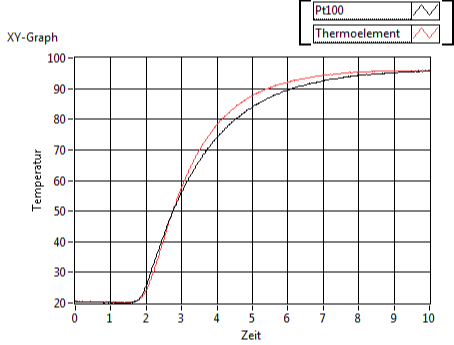
\includegraphics[scale=1]{Bilder/temperaturverhalten.png}
\caption{Temperaturverhalten}
\end{figure}
\end{center}
Berechnung $t_{90}$ und $t_{10}$:\\
\begin{center}
$\Delta t_{Pt100} = t_{Pt100_{max}} - t_{Pt100_{min}} = 96^\circ C - 20,3^\circ C = 75,7^\circ C$\\
$\Delta t_{Thermo} = t_{Thermo_{max}} - t_{Thermo_{min}} = 95,8^\circ C - 20,5^\circ C = 75,3^\circ C$\\
\vspace{0.5cm}
$T(t_{Pt100_{10}}) = \Delta t_{Pt100} \cdot 10\% + t_{Pt100_{min}}$\\
$T(t_{Pt100_{10}}) = 75,7^\circ C \cdot 10\% + 20,3^\circ C = 27,87^\circ C$\\
$=> t_{Pt100_{10}} = 5,11s$\\
\vspace{0.5cm}
$T(t_{Thermo_{10}}) = \Delta t_{Thermo} \cdot 10\% + t_{Thermo_{min}}$\\
$T(t_{Thermo_{10}}) = 75,3^\circ C \cdot 10\% + 20,5^\circ C = 28,03^\circ C$\\
$=> t_{Thermo_{10}} = 5,12s$\\
\vspace{0.5cm}
$T(t_{Pt100_{90}}) = \Delta t_{Pt100} \cdot 90\% + t_{Pt100_{min}}$\\
$T(t_{Pt100_{90}}) = 75,7^\circ C \cdot 90\% + 20,3^\circ C = 88,43^\circ C$\\
$=> t_{Pt100_{90}} = 2,14s$\\
\vspace{0.5cm}
$T(t_{Thermo_{90}}) = \Delta t_{Thermo} \cdot 90\% + t_{Thermo_{min}}$\\
$T(t_{Thermo_{90}}) = 75,3^\circ C \cdot 90\% + 20,5^\circ C = 88.27^\circ C$\\
$=> t_{Thermo_{90}} = 2,075s$\\
\end{center}
Ansprechzeit:\\
\begin{center}
$t_{Pt100_{An}} = t_{Pt100_{90}} - t_{Pt100_{10}}$\\
$t_{Pt100_{An}} = 5,11s-2,14s=2,97s$\\
\vspace{0.5cm}
$t_{Thermo_{An}} = t_{Thermo_{90}} - t_{Thermo_{10}}$\\
$t_{Thermo_{An}} = 5,12s-2,075s = 3,045s$\\

\end{center}

Berechnung $\tau$:\\
\begin{center}
$\tau_{Pt100} = \frac{t_{Pt100_{An}}}{ln(9)}$\\
$\tau_{Pt100} = \frac{2,97s}{ln(9)} = 1,352s$\\
\vspace{0.5cm}
$\tau_{Thermo} = \frac{t_{Thermo_{An}}}{ln(9)}$\\
$\tau_{Thermo} = \frac{3,045s}{ln(9)} = 1,386s$\\
\end{center}

\newpage

Berechnung $t_{0,90}$:\\

\begin{center}
$t_{Pt100} = -ln(0,1)\cdot \tau_{Pt100}$\\
$t_{Pt100} = -ln(0,1)\cdot 1,352s = 4,50s$\\
\vspace{0.5cm}
$t_{Thermo} = -ln(0,1)\cdot \tau_{Thermo}$\\
$t_{Thermo} = -ln(0,1)\cdot 1,386s = 4,58s$
\end{center}


\subsection{Fazit}
Es ist zu erkennen, dass die Kennlinien, trotz etwas größeren Differenzen zwischen 3 und 8 Sekunden, nahezu gleich sind. Bei ungefähr 10 Sekunden befinden sich der Pt100 und das Thermoelement bei fast exakt der selben Temperatur. Auch anhand sehr ähnlichen Ergebnissen der Berechnungen ist festzustellen, dass sich Pt100 und das Thermoelement sehr ähneln. \\
Somit ist zu dem Entschluss zu kommen, dass sich beide Bauelemente zur Temperaturmessung sehr gut eignen. 

\end{document}
